% Contesto applicativo

% Stato dell'arte

% Storia e motivi, tutte le volte che il metaverso è stato proposto alla gente e tutte le tecnologie che sono attualmente in uso e anche samsung con il suo vr set del cellulare

\section{Il Metaverso}

    Il concetto di Metaverso nasce nella letteratura di fantascienza, infatti il termine fu coniato da Neal Stephenson nel suo libro \textit{Snow Crash} del 1992. 
    %
    Il termine descriveva uno spazio tridimensionale dove la realtà si univa con un mondo virtuale costantemente attivo.
    %
    Nonostante questo concetto non sia recente, saper dare una definizione di cosa è il Metaverso genera molte difficoltà, infatti è una tecnologia che per la maggior parte ancora non esiste e sebbene riusciamo a ragionare su esperienze tecnologiche future siamo ancora lontani dal renderla possibile.
    %
    Ancora non possiamo sapere quali caratteristiche saranno più importanti e che tipo di dinamiche guideranno la sua formazione, come negli anni '80 era difficile descrivere cosa sarebbe stato internet nel 2022, allo stesso modo è difficile saper descrivere il Metaverso.
    %
    Ad oggi si può dire che il Metaverso è il nuovo principale obiettivo delle grandi compagnie di tecnologia mondiali, come Facebook - non a caso rinominata \textit{Meta} - e Epic Games - azienda proprietaria del motore grafico Unreal Engine e di Fortnite, il videogioco che ad oggi viene considerato la piattaforma più vicina al Metaverso che sia stata fatta.

    % Definire meglio chi è Matthew Ball
    Matthew Ball, CEO di Epyllion e scrittore di \textit{The Metaverse and How it Will Revolutionize Everything}, lo definisce in questo modo \cite{Ball2022}: 

    \begin{displayquote}
        \textit{Io definisco il metaverso come un network ampiamente scalabile e interoperabile di mondi virtuali 3D renderizzati in tempo reale che possono essere vissuti, in modo sincrono e persistente, da un numero infinito di user effettivi, ciascuno con un senso di presenza individuale, supportando al contempo continuità di dati quali cronologia, identità, comunicazione, pagamenti, diritti e oggetti.}
    \end{displayquote}

    Secondo Matthew Ball il Metaverso è quindi una combinazione di molte tecnologie diverse che collaborano per costruire un'esperienza continua e persistente.
    %
    È l'unione di mondi virtuali, tecnologie - quali visori per la realtà virtuale, dispositivi indossabili e camere a proiezione 3D - e internet.
    %
    È una nuova era della tecnologia che verrà costruita iteramente e lentamente al di sopra delle infrastrutture e dei protocolli esistenti che verranno migliorati o sostituiti in base alle esigenze.
    %
    Un ruolo fondamentale lo avranno le piattaforme virtuali, esse infatti daranno effettivamente vita ai mondi virtuali in cui le persone potranno entrare.
    %
    Alcune di queste hanno scopi puramente di intrattenimento - come Roblox, The Legend of Zelda o Minecraft - altri hanno intenti accademici e professionali - come Osso VR o come i simulatori di volo per l'addestramento di piloti.

    % La storia del Metaverso è perciò la storia di tutte le piattaforme online e di tutte le tecnologie che stanno contribuendo a costruire mondi ed esperienze virtuali.

    \subsection{Storia del metaverso}
    Sebbene il termine fu coniato nel 1992, il concetto di Metaverso affonda le radici nella letteratura Cyberpunk.
    %
    Tale letteratura comprende romanzi come \textit{True Names di Vernor Vinge} del 1981, che descrive quello che può essere considerato il primo esempio di cyber-spazio, e \textit{Neuromancer di William Gibson} nel 1985, che invece descrive un cyber-spazio dalle caratteristiche molto simili al Metaverso che intendiamo oggi.

    Il primo dei due libri è particolamente importante perché è citato come fonte di ispirazione per il primo gioco nel Metaverso: Habitat \cite{Habitat1990}.

        \subsubsection{Habitat - la prima implementazione di Cyber-spazio}

        
        Habitat viene definito dai creatori un \textit{ambiente virtuale online multigiocatore} \cite{Habitat1990}, ogni utente utilizzava il proprio Personal Computer come frontend comunicando su un network a commutazione di pacchetto con un sistema back-end centralizzato.
        %
        La prima versione di Habitat era stata sviluppata per il Commodore 64 nel 1985 e non era possibile avere stanze virtuali popolose né grafica 3D a causa delle limitate risorse che il modello offriva.
        %
        Nonostante questo, Habitat rese possibile per la prima volta a persone da tutto il mondo di incontrarsi in uno spazio virtuale.
        %
        Gli utenti avevano una rappresentazione virtuale di se stessi in terza persona, questa rappresentazione venne chiamata avatar, come nel romando \textit{True Names}.
        %
        L'utente, attraverso il proprio avatar, aveva la possibilità di interagire con oggetti, parlare con altri avatar attraverso una chat che appariva a schermo in stile "word baloon" e muoversi nel mondo di Habitat composto da un grande numero di posizioni che venivano chiamate \textit{Regioni}.

        \begin{figure}[!ht]
            \centering
            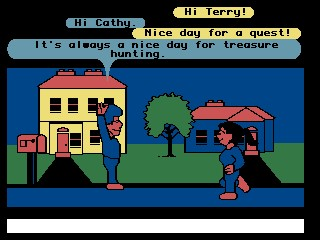
\includegraphics[width=5cm]{figure/lessonshabitat.jpg}
            \caption{Una tipica scena in Habitat.}
        \end{figure}

        Habitat fu un importante progetto che fece capire agli sviluppatori le difficoltà nell'approciarsi alla creazione di un ambiente virtuale multigiocatore e lasciarono in eredità un testo con le lezioni principali che impararono. \cite{Habitat1990}
         
        \subsubsection{Second Life}

        Un altro importante esempio di cyber-spazio è Second Life, una piattaforma online lanciata nel 2003 dalla società Linden Lab.
        %
        Second Life è un ambiente virtuale online multigiocatore 3D e  gli utenti sono rappresentati digitalmente attraverso un avatar tridimensionale.
        %
        Attraverso gli avatar gli utenti hanno la possibilità di socializzare con altri utenti, sia attraverso chat testuale che vocale, esplorare il mondo virtuale, composto da migliaia di regioni chiamate \textit{Sim} e partecipare ad attività di vario genere come concerti, raduni e lezioni e molto altro.
        %
        La particolarità di questa piattaforma, che la distingue da altri videogiochi 3D, è che il contenuto del mondo di gioco viene interamente creato dai giocatori e non c'è un obiettivo da perseguire né una storia.
        %
        Inoltre Second Life possiede una sua economia interna e un token virtuale a circuito chiuso chiamato \textit{Linden Dollar L\$}. 
        %
        Questa valuta non ha valore monetario ma può essere scambiata con Linden Lab per un corrispettivo in dollari.
        %
        Essa può essere usata per comprare, vendere, affittare o commerciale beni e servizi con altri giocatori all'interno del mondo di gioco.
        
        In Second Life per la prima volta brand e organizzazioni parteciparono alla realizzazione di oggetti ed eventi nel mondo virtuale portando il gioco ad evolversi e distaccarsi dall'essere una pura esperienza d'intrattenimento. 
        %
        Brand come Adidas, Calvin Klein e Lacoste lanciarono linee di vestiti indossabili dagli avatar dei giocatori \cite{Fascion2nd} mentre alcune università hanno usato Second Life con obiettivi educativi e formativi, incluse l'Università di Harvard e di Oxford \cite{University2ndLife} ma anche alcune italiane come le università di Milano, di Torino, di Salerno e di altre città. \cite{UnitoIn2ndLife, 2ndLifeWikipedia} 
        %
        Un altro evento importante fu lo sciopero dei lavoratori IBM organizzato su Second Life nel 2007, durante questo sciopero migliaia di avatar contemporaneamente si radunarono per protesta sulla Sim dell'azienda. \cite{2ndLifeWikipedia}
        
        \subsubsection{I visori per la realtà aumentata e virtuale} % qui mettererei i tentativi di samsung

        %Costruzione???
        Un importante contributo alla costruzione del Metaverso lo dobbiamo all'avanzamento tecnologico dei dispositivi per la realtà aumentata (AR) e per la realtà virtuale (VR).
        %
        Questa tecnologia ha accompagnato il concetto del Metaverso sin dai suoi albori.
        %
        %Infatti, troviamo dispositivi simili in \textit{Snow Crash} ma anche nel più recente \textit{Ready Player One}.

        I visori per la realtà aumentata e per la realtà virtuale sono un avanzamento di un dispositivo ottico più antico, lo stereoscopio. 
        %
        Inventato nella prima metà dell'800, lo stereoscopio simula la tridimensionalità del mondo reale per come viene percepita dagli occhi umani. 
        %
        Infatti gli occhi umani trasmettono al cervello due immagini della stessa scena con due punti di osservazione leggermente diversi.
        %
        Il cervello sovrapponendo le due immagini riesce a valutare la distanza degli oggetti: più un oggetto è scostato nelle due immagini più esso viene percepito come vicino, al contrario minore lo scostamento, maggiore è la distanza percepita \cite{Stereoscopia}.
        %
        Lo stereoscopio permette di far vedere a ciascun occhio una tra due immagini molto simili tra loro, realizzate appositamente per essere percepite dal cervello umano come se fosse un singolo punto di vista reale.
        %
        Questo conferisce al soggetto la tridimensionalità desiderata.

        \begin{figure}[!ht]
            \centering
            %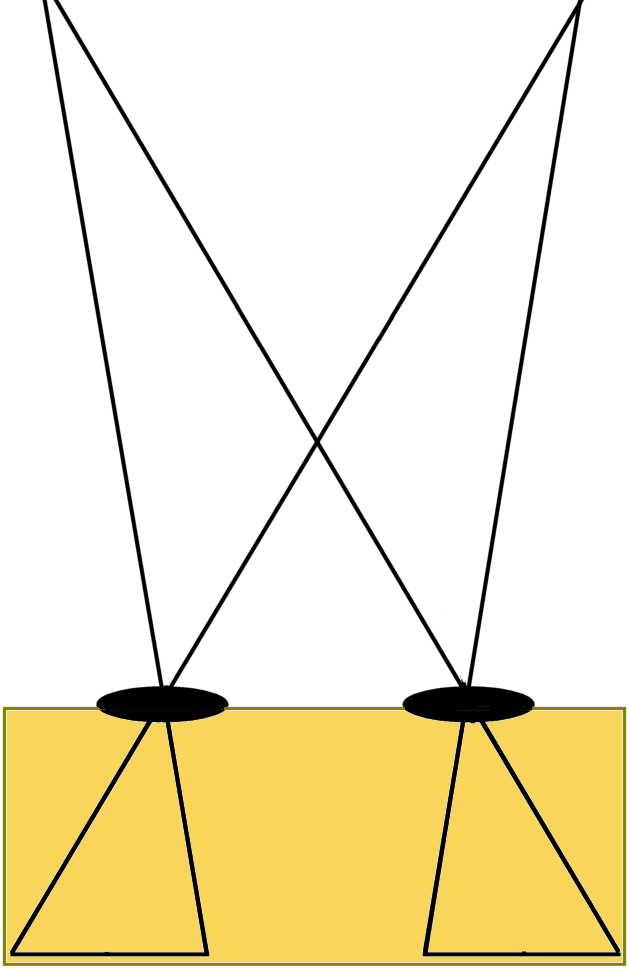
\includegraphics[width=5cm, angle=90]{figure/Stereocamera.png}
            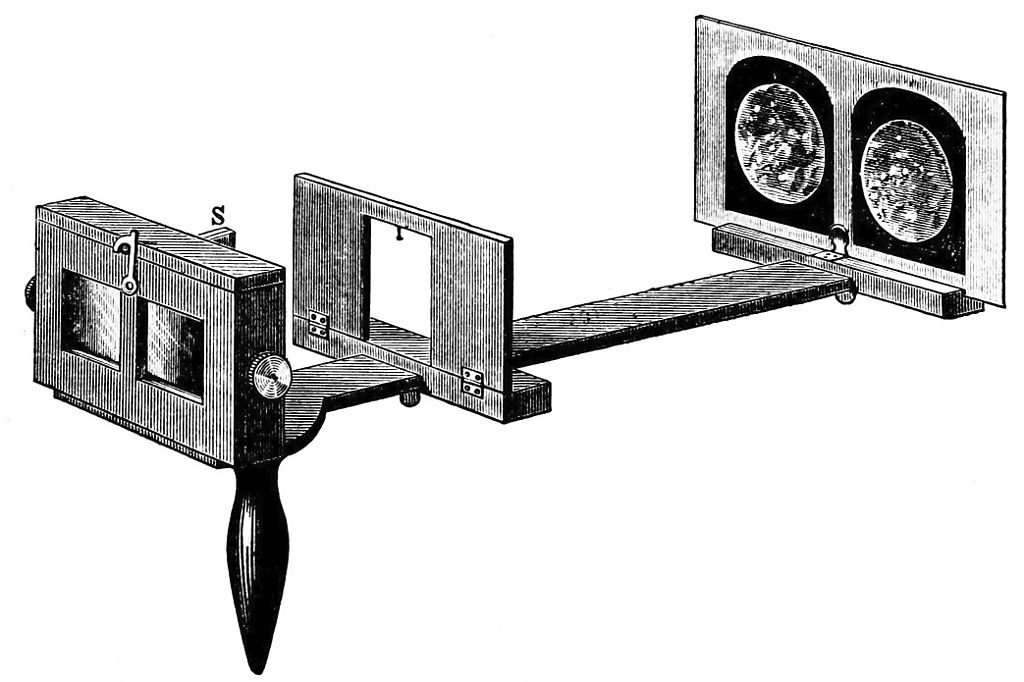
\includegraphics[height=5cm]{figure/Stereoscopia.jpg}
            \caption{Stereoscopio statunitense regolabile.}
        \end{figure}

        Il primo a sfruttare questo principio per immergersi in una realtà simulata fu Ivan Sutherland nel 1968.
        %
        Insieme ai suoi studenti, egli creò il primo sistema di realtà virtuale con visore che permetteva di osservare un ambiente virtuale renderizzato in wire-frame model (metodo che disegna solo gli spigoli di un oggetto 3d).
        %
        Il visore era così pesante che doveva essere appeso al soffito, per questo fu battezzato \textit{La spada di Damocle}.

        Dagli anni '70 fino agli anni '90 i dispositivi AR/VR furono designati quasti esclusivamente per scopi medici, simulazioni di volo, progettazione nell'industria automobilistica e addestramento militare \cite{70and90VR}.
        %
        Bisogna aspettare fino al 1991 per assistere al primo visore VR lanciato sul mercato, ossia quando l'azienda Virtuality Group lanciò la serie 1000 dei prodotti Virtuality che girava sul Commodore Amiga 3000.
        %
        Oltre ai prodotti Virtuality, gli anni '90 videro altre aziende puntare su questa tecnologia, come Sega con l'annuncio del Sega VR e la Nintendo con il lancio del Virtual Boy.

        Dopo allora l'interesse verso i visori da parte di grandi aziende è stato modesto fino al 2010, anno in cui venne prodotto il primo prototipo dell'Oculus Rift.
        %
        Questo visore aveva il tracciamento della posizione, godeva di un angolo di visione di 90° e risolveva i problemi di distorsione che avevano i precedenti visori pre-distorcendo l'immagine renderizzata in tempo reale.
        %
        Inoltre, nel 2013 l'azienda Valve inventò un display a bassa latenza che permise di creare schermi privi di lag e di motion blur indesiderato (il cosiddetto \textit{"smear-effect"}).
        %
        Questo in aggiunta all'avanzamento tecnologico di vari componenti sviluppati per smartphone - giroscopi, sensori di movimento, piccoli schermi HD e processori potenti miniaturizzati - diedero nuova linfa a questa tecnologia e vennero lanciati sul mercato molti modelli di visori.

        
        Nel 2014 Google annunciò Cardboard, una piattaforma per la realtà virtuale fruibile con lo smartphone inserito all'interno di un visore.
        %
        Un simile progetto lo distribuì Samsung nel 2015 con Samsung Gear VR.
        %
        Entrambi i progetti non offrivano un'esperienza coinvolgente e, nonostante fossero economici, non riscossero il successo desiderato e vennero dismessi. 
        %
        Nel 2016 Valve e l'azienda HTC lanciarono il visore HTC Vive.
        %
        Questo apparecchio sfruttava una nuova tecnologia chiamata \textit{"room scale"} che permetteva all'utente di muoversi liberamente in una zona di gioco invece di essere vincolato a stare fermo, inoltre i controller erano tracciati grazie a telecamere montate sul visore stesso e grazie ad una serie di sensori che andavano montati nella stanza.
        %
        Sempre nel 2016 l'azienda Sony lanciò il Playstation VR, visore che montava un pannello OLED a 1080p e aveva un angolo di visuale di 100°.
        %
        Questo visore non godeva di componenti di rilievo in confronto ai competitor ma si affacciava ad un mercato diverso, quello delle console. 

        Aggiungere una conclusione!

    \subsection{Stato dell'arte - Building the Metaverse}

    Oggi parlando di Metaverso si fa riferimento a piattaforme che riescono ad avvicinarsi ma che ancora non sono il Metaverso come definito in precedenza.
    %
    Piattaforme come Roblox, Fortnite e Horizon Worlds presentano molti elementi del Metaverso, come una consistente rappresentazione 3D degli utenti, come la possibilità per gli utenti di creare i contenuti e come la possibilità di portare queste in una moltitudine di esperienze diverse. 
    %
    Questi \textit{"giochi"} combinano insieme tante tecnologie e provano a produrre un esperienza che si discosta da tutto ciò che è venuto prima. Ma per avere il Metaverso descritto da Matthew Ball ci vorranno ancora anni di ricerca e sviluppo. 
    %
    Infatti mancano ancora i protocolli, le innovazioni che possono permettere quella visione e soprattutto le tecnologie necessarie.
    
    A livello infrastrutturare le tecnologie per accomodare migliaia o addirittura milioni di persone allo stesso momento in un'esperienza sincrona e persistente semplicemente non esistono.
    %
    E non solo, internet non è stato progettato per permettere esperienze simili.
    %
    La maggior parte delle connessioni che avvengono sfruttano il protocollo TCP che garantisce la qualità dei dati ricevuti ma permette solo connessioni singole tra due utenti.
    %
    In effetti è quello che sperimentiamo quando inviamo una mail o ci connettiamo su Facebook.
    %
    Avvengono milioni di connessioni singole simultaneamente nel mondo ma è tutt'oggi molto difficile permettere a più di un centinaio di utenti di essere connessi tra di loro con connessioni full-duplex.
    %
    Per garantire un'esperienza sincrona, il Metaverso avrebbe invece bisogno proprio di questo tipo di infrastruttura, un sistema simile alle attuali videochiamate o alle connessioni che avvengono all'interno dei videogiochi online ma in scala molto più grande.
    %
    Le attuali piattaforme virtuali nascondono questa mancanza dividendo il loro mondo virtuale in diverse zone o partite, ognuna connessa con un server e con un numero finito di utenti, e mascherano il passaggio dell'utente da un server ad un altro come un passaggio tra queste divisioni.
    %
    %Molte aziende stanno lavorando per risolvere questo problema tra cui l'azienda Improbable \cite{Ball2020}.

    Per garantire l'interoperabilità e la sincronia inoltre, il Metaverso avrà bisogno di un largo e complesso insieme di nuovi protocolli e standards.
    %
    Infatti i sistemi attuali operano su formati simili ma non compatibili tra loro (basti pensare ai numerosi standard per la compressione d'immagini che sono presenti in internet).
    %
    Questo è mitigato dal fatto che l'attuale esperienza di internet è asincrona, perciò quando un contenuto viene migrato da un sistema ad un altro viene spesso convertito nel formato di destinazione durante la fase non connessa.
    %
    % Ad esempio, inserendo un immagine con formato .bmp sul client di Whatsapp questa viene automaticamente convertita in formato .jpeg in modo da poter essere inviata attraverso i protocolli utilizzati dal servizio di messaggistica.
    %
    La difficoltà di questo passaggio è causata dalla naturale resistenza che hanno aziende e organizzazioni diverse a collaborare per creare uno standard condiviso, un esempio di ciò è come Apple sia resistente ad adottare lo standard USB-C sui suoi dispositivi o anche come siano presenti un gran numero di standard per le prese di corrente nel mondo.

    Perciò Matthew Ball immagina che il Metaverso arriverà, similmente per come è stato con internet, come un disordinato insieme di processi e sviluppi diversi che gradualmente si uniformerà.
    %
    La differenza sostanziale è che internet si sviluppò in ambito universitario e aveva come scopo quello di mettere in comunicazione le facoltà sparse nel mondo.
    %
    Al contrario in questo momento storico è l'industria privata che detiene la consapevolezza del potenziale del Metaverso, le risorse economiche ed ingegneristiche per svilupparlo e tutto l'interesse a far si che questo divenga realtà.

        \subsubsection{Epic Games} \label{EpicGames}

        Una delle caratteristiche più importanti che deve avere il Metaverso secondo Ball è quella di essere un ambiente attraente per gli utenti e le aziende.
        %
        Quello che ad oggi si è avvicinato di più a questo scopo è il gioco Fortnite.
        %
        Sviluppato e distribuito da Epic Games, questo gioco nel tempo, e grazie alla sua fama, è diventato un occasione di incontro e di socialità, ma soprattutto si è avvicinato al concetto di Metaverso in quanto il mondo virtuale di gioco è diventato luogo di eventi sociali indipendenti dal gioco stesso quali concerti e luogo di visione di contenuti multimediali a cui gli utenti possono assistere con il proprio avatar.
        %
        Nella piattaforma, infatti, si sono svolti concerti di artisti famosi come Marshmellow, Ariana Grande e Trevis Scott e sono stati distribuiti i trailer di Star Wars e di Tenet in anteprima.

        Fortnite inoltre è una delle poche piattaforme che presenta livelli di interoperabilità così elevati. 
        %
        Infatti, Fortnite si interseca con varie proprietà intellettuali di aziende quali la Marvel, la DC, la Sony, è accessibile attraverso dispositivi concorrenti (iPhone, Android, Playstation, Xbox e computer) e include anche diversi sistemi di identità e pagamento.

        Inoltre Epic Games è proprietaria del secondo game engine più utilizzato del settore: Unreal Engine.
        %
        Questo engine nel tempo è diventato così completo e realistico che ha iniziato a venir usato anche per grosse produzioni hollywoodiane, come \textit{The Mandalorian}, ma anche per progetti di architettura urbana, per progettazione di automobili e per esercitazioni militari simulate dell'esercito degli Stati Uniti e del Regno Unito \cite{Ball2022, BallUnreal,USMilitaryUnreal}.
        %
        Tutto questo rende il loro sistema potenzialmente già compatibile con centinaia di contenuti velocizzando il processo di migrazione di applicativi all'interno del Metaverso.

        \begin{figure}[h!]
            \centering
            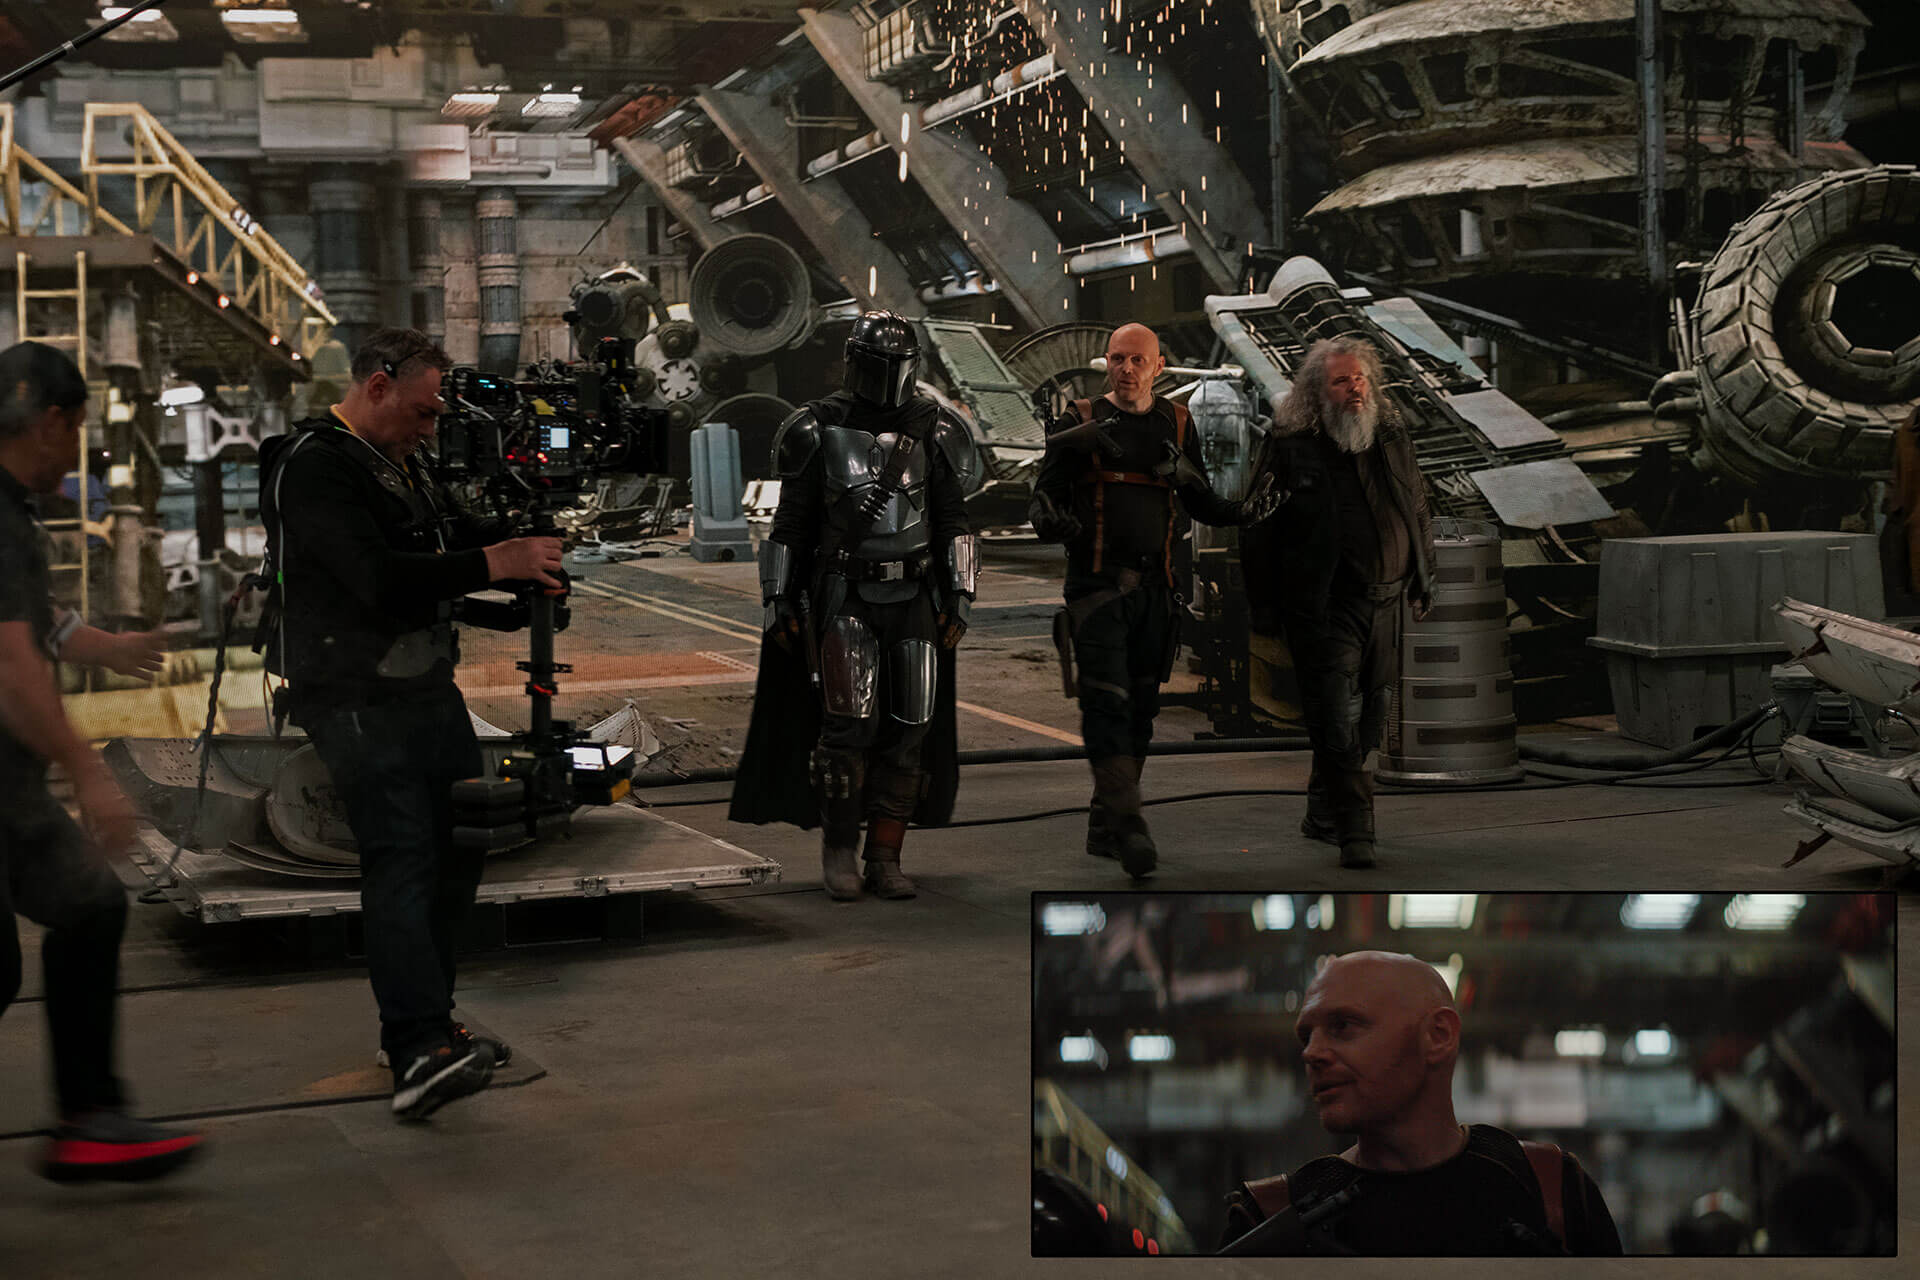
\includegraphics[height=6cm]{figure/TheMandalorianUnreal.jpg}
            \caption{Set di The Mandalorian con scenografia renderizzata con Unreal Engine}
        \end{figure}

\section{Il motore grafico Unreal Engine 5}

Come anticipato nel capitolo \ref{EpicGames}, Unreal Engine è un motore grafico 3D sviluppato da Epic Games.
%
La prima versione del software fu sviluppata interamente da Tim Sweeney, il fondatore della società, dal suo garage. Tim Sweeney iniziò lo sviluppo nel 1995 e il motore grafico debuttò con un videogioco chiamato \textit{Unreal}, sviluppato da Cliff Bleszinski e James Schmalz, nel 1998.
%
Nonostante né il motore grafico né il gioco fossero completati del tutto, Unreal ottenne il successo desiderato anche grazie a una fedele community che utilizzando l'UnrealScript (il codice proprietario sviluppato da Sweeney per il game engine) espanse il gioco e rese Epic MegaGames (poi rinominata Epic Games) un nome importante nell'industria videoludica.
%
Inoltre il gioco fu anche la vetrina desiderata per l'engine che da quel momento fu utilizzato sotto licenza da altri sviluppatori che portarono Unreal Engine a diventare un motore grafico apprezzato ed accreditato nel settore \cite{PolygonUnreal, UHistory}.
%
%Unreal Engine è il motore grafico utilizzato per alcune delle uscite videoludiche più importanti degli anni 2000, quali Gears of War, BioShock, Deus Ex e Tom Clancy's Splintel Cell.
%

Unreal Engine fu lanciato poco prima il passaggio alle schede grafiche dedicate.
%
Questo ha fatto si che la prima versione si basava totalmente sul software rendering, ossia sfruttava unicamente la CPU. 
%
Sweeney sviluppò l'editor di Unreal engine in Visual Basic e prese fortemente ispirazione dall'ambiente di lavoro di quest'ultimo per l'interfaccia utente, soprannominò l'editor Unrealed.
%
Infatti già dalle prime versioni di Unreal Engine c'erano dei moduli che si potevano trascinare nella scena direttamente, poi una volta nella scena bastava fare un doppio click su di essi per far comparire l'editor di testo e poter scrivere il codice desiderato \cite{InterviewSweeney}.

\begin{figure}[h!] 
    \begin{center}
    \begin{tabular}{c @{\hspace{1em}} c}
    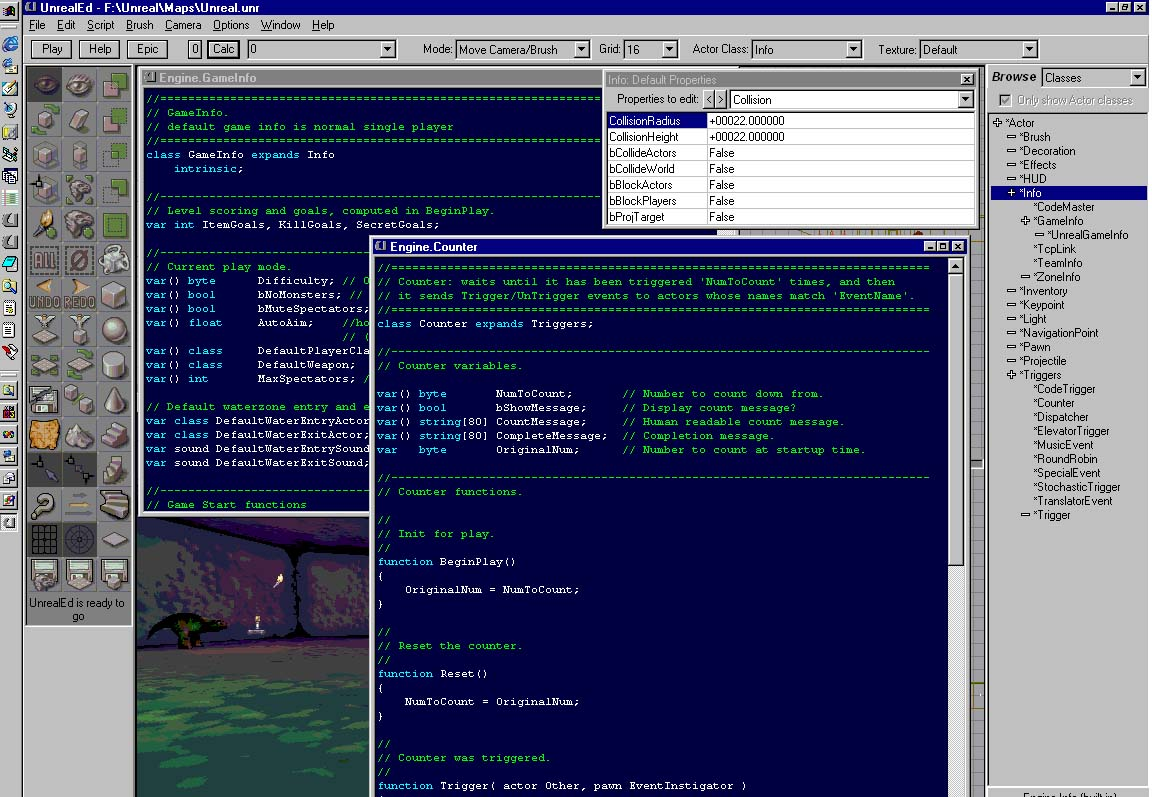
\includegraphics[width=6.5cm]{figure/UnrelEngineEditor1.jpg} &
    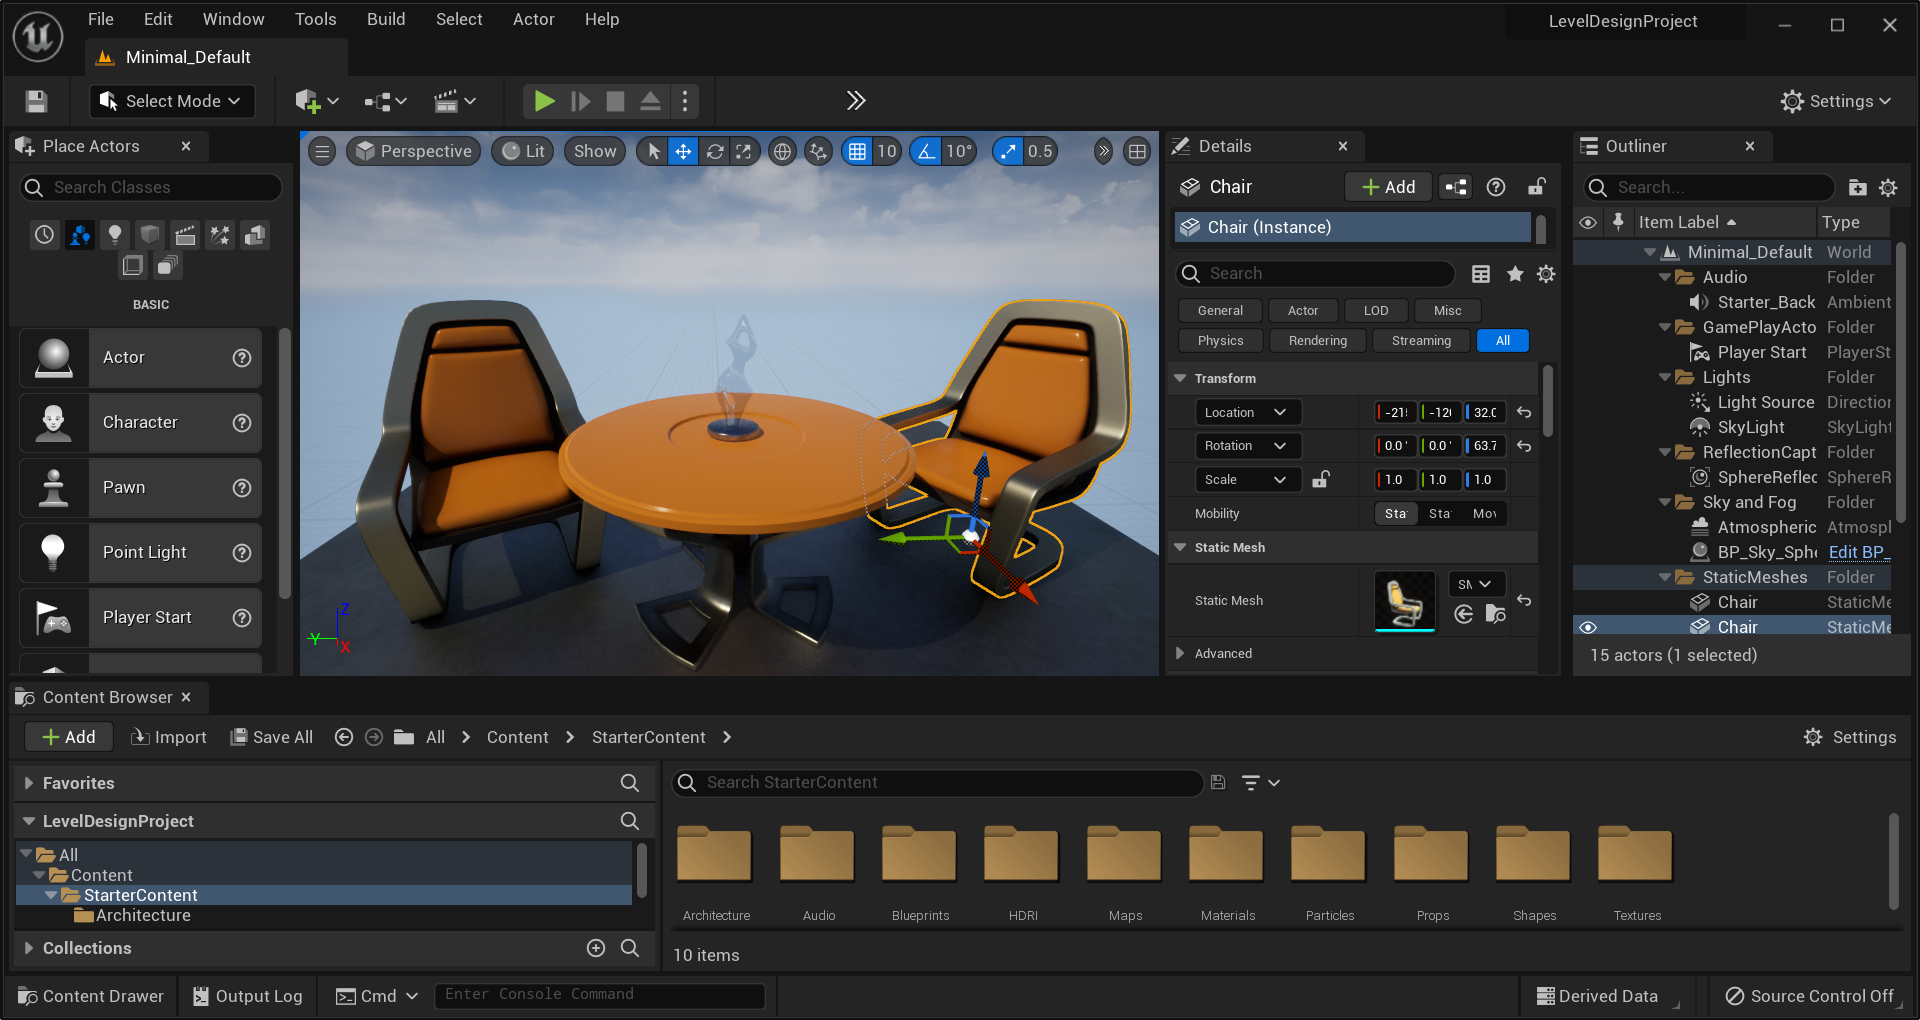
\includegraphics[width=6.5cm]{figure/01-level-editor-windows.png} \\
     (a) & (b)
    \end{tabular}
    \end{center}
    \caption{Screenshot della prima versione di UnrealEd. (a) Screenshot della versione 5 dell'editor di Unreal Engine. (b)} \label{fig:figura-doppia}
\end{figure}

Ad oggi il motore grafico ha abbandonato sia UnrealScript che Visual Basic ma le scelte iniziali sono rimaste.
%
Infatti le classi native che troviamo oggi nella libreria Unreal C++ sono le stesse che c'erano in UnrealScript.
%
Sono ancora presenti le classi native principali Actor, Pawn e Character: la classe Actor è la classe base per tutti gli oggetti che vengono disposti o vengono generati nel livello; la classe Pawn è un'espansione della classe Actor per tutti gli oggetti che posso essere governati da giocatori o dall'intelligenza artificiale; la classe Character è un'espansione della classe Pawn che possiede una Mesh, delle Collisions e una logica di movimento incorporata. 
%
Alla creazione di una classe l'editor fa scegliere la parent class e in base alla scelta viene generato automaticamente il rispettivo script di base \cite{UProgrIntro}.

\begin{lstlisting}[caption = File header generato alla creazione di un Actor]
    #include "GameFramework/Actor.h"
    #include "MyActor.generated.h"

    UCLASS()
    class AMyActor : public AActor
    {
        GENERATED_BODY()

    public:

        //Sets default values for this actor's properties
        AMyActor();

        //Called when the game starts or when spawned
        virtual void BeginPlay() override;

        //Called every frame
        virtual void Tick(float DeltaSeconds) override;

    };
\end{lstlisting}

È possibile inoltre esporre una variabile dello script all'editor tramite appositi specificatori, espandibili con una lista di proprietà tra cui scegliere:

\begin{lstlisting}[caption = Specificatore UPROPERTY per esporre una variabile all'editor]
    UPROPERTY(EditAnywhere, category="VariableCategory")
    int32 MyVariable;
\end{lstlisting}

Anche l'impostazione iniziale organizzata in moduli è stata mantetuta.
%
I moduli sono gli oggetti che possono essere trascinati in scena e che hanno funzionalità definite.
%
È possibile espandere la lista di oggetti trascinabili in scena con quelli personalizzati dallo sviluppatore, si troveranno nel Content Browser e non nel pannello di Place Actor.

In Unreal Engine la scena nel quale viene creata l'esperienza di gioco è chiamata Level.
%
Un Level è un ambiente 3D che può essere popolato da oggetti e geometrie.
%
Ogni oggetto che viene posizionato nel Level è un Actor.
%
Più tecnicamente infatti un Actor è la classe che definisce un qualsiasi oggetto a cui è associato un Transform, ossia l'informazione sulla posizione, sulla rotazione e sulla scala \cite{ULevelEditor}.

L'interfaccia utente è composta da diverse finestre ed è altamente personalizzabile.
%
Alla prima accensione dell'engine viene proposto il layout di default.

\begin{figure}[h!]
    \centering
    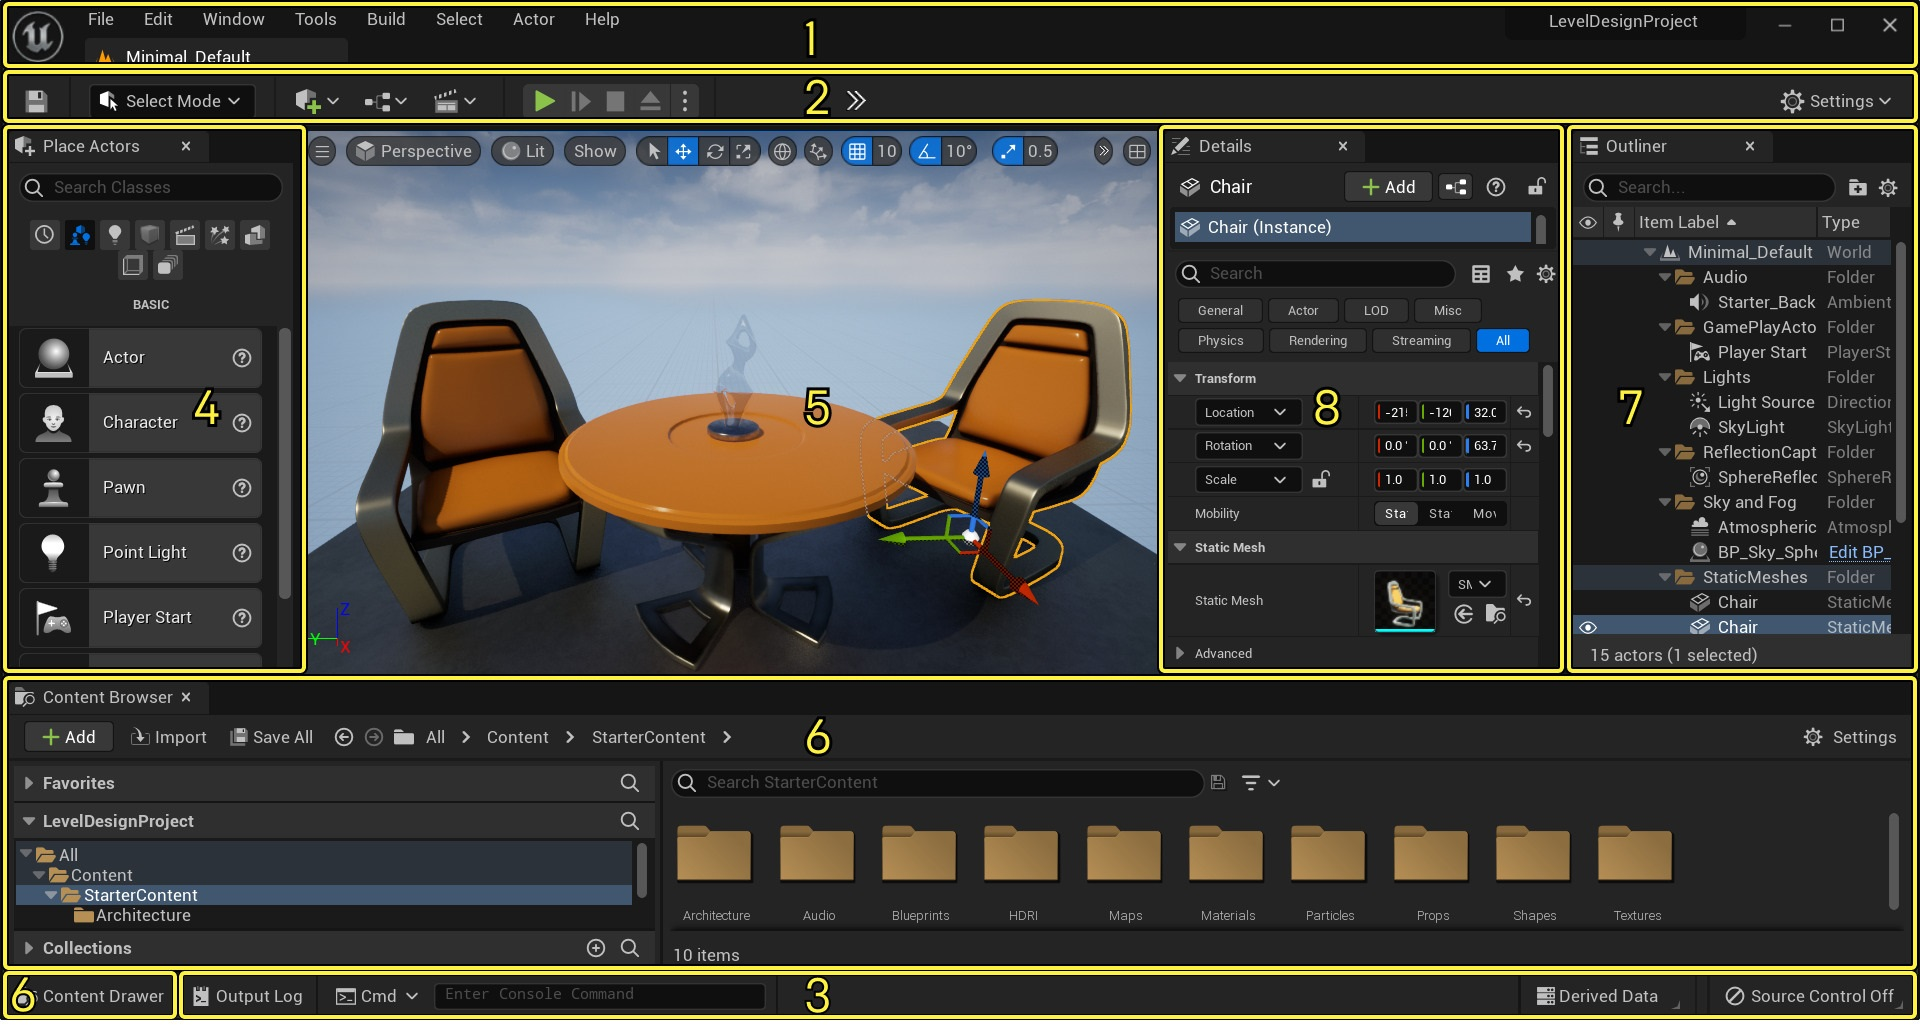
\includegraphics[height=6cm]{figure/02-default-interface-windows.jpg}
    \caption{Interfaccia di default di Unreal Engine 5}
\end{figure}

\begin{description}
    \item [1. Tab Bar and Menu Bar:] Il Lever Editor ha delle schede simili a quelle che hanno i browser in alto. Infatti oltre al livello si possono navigare tutti i tipi di oggetti singolarmente e qui possono essere raggruppate tutte le schede. \\ La Menu Bar offre accesso agli strumenti generali dell'editor quali le impostazioni del progetto e le preferenze.
    \item [2. Toolbar:] Questo pannello mostra un gruppo di comandi, offrendo così rapido accesso agli strumenti e alle funzionalità più utilizzate.
    \item [3. Buttom Toolbar:] Contiene scorciatoie per la Console di comando, per l'Output Log e per la funzionalità di Delivered Data 
    \item [4. Place Actor / Modes:] Il Lever Editor può essere messo in diverse modalità attivando specifice interfacce di editing per particolari tipi di azioni che si vogliono compiere nel livello. Le possibili modalità sono:
    \begin{itemize}[-]
        \item Select: per selezionare, spostare e aggiungere attori nella scena.
        \item Landscape: per la creazione e la modifica di vaste aree di terreno.
        \item Foliage: per la creazione e la modifica di un alto numero di istanze di Static Mesh per la popolazione della scena con elementi naturali 
        \item Mesh Paint: per la pittura di vertici e texture su Static Mesh direttamente nella Viewport.
        \item Modeling: per la creazione di mesh poligonali semplici 
        \item Fracture: per la creazione di oggetti e ambienti distruttibili
        \item Brush Editing: per la modifica della geometria delle mesh.
        \item Animation: per creare e modificare animazioni.
    \end{itemize}
    \item [5. Viewports:] questo pannello è la finestra verso il mondo che l'utente sta creando. Permette di selezionare, spostare, ruotare e scalare gli oggetti direttamente con il mouse e di muovere il punto di vista all'interno della scena. 
    \item [6. Content Browser / Content Drawer:] permette di visualizzare tutti gli asset di gioco e di organizzarli in cartelle
    \item [7. Outliner:] permette di visualizzare e selezionare tutti gli attori presenti nella scena in una vista gerarchica ad albero.
    \item [8. Details:] questo pannello contiene le informazioni, le funzionalità e le utilità degli oggetti che vengono selezionati. Contiene i box per la modifica dei dati del Transform per muovere, ruotare o scalare gli oggetti e mostra tutte le proprietà editabili in base al tipo di attore che si seleziona. È qui che vengono visualizzate le variabili esposte all'editor dallo script in C++.
\end{description}

Unreal Engine permette di aggiungere funzionalità a classi già presenti del motore tramite le classi Blueprints.
%
Esse permettono di raggruppare componenti di tipologie diverse, chiamati appunto Components, sotto un'unica classe e di espandere le loro funzionalità attraverso la programmazione.
%
In Unreal Engine la programmazione può essere implementata sia attraverso C++ che attraverso la programmazione visiva organizzata a nodi dei Blueprints, chiamata Blueprints Visual Scripting. 
%
Il vantaggio della Blueprints Scripting è che è di veloce implementazione soprattutto per i principianti della programmazione. 
%
D'altro canto però questa programmazione visiva non da libero accesso al codice di gioco, è meno flessibile e meno efficiente della programmazione C++.
%
Invece, lo svantaggio principale di C++ è che è molto più facile commettere errori che compromettono l'intero engine.
%
Infatti bisogna fare particolare attenzione all'utilizzo dei puntatori, e delle funzioni che li sfruttano, perché l'utilizzo di uno di questi ancora non inizializzato porterà ad una \textit{null pointer exception} e al conseguente crash dell'engine.
%
Inoltre, questo tipo di errori sono spesso di difficile interpretazione.

\begin{figure}[h!]
    \centering
    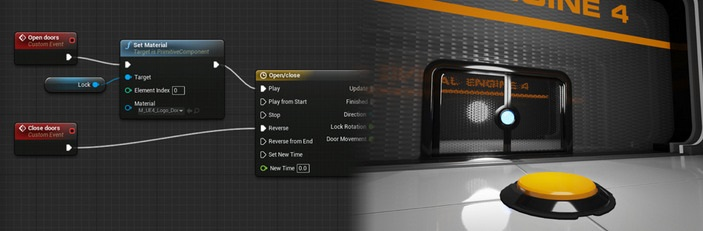
\includegraphics[height=3cm]{figure/BlueprintClass.jpg}
    \caption{Esempio di classe Blueprint per l'apertura e la chiusura di una porta in gioco}
\end{figure}

Aggiungere una conclusione!

\section{Il software di modellazione Blender}

Blender è un un software per la creazione di contenuti 3D gratuito e \textit{open source}.
%
Supporta l'intera pipeline di strumenti per il 3D - modellazione, rigging, animazioni, creazione e pittura di texture, simulazioni, rendering, compositing e motion tracking.
%
È un software cross-platform, è disponibile per Linux, Windows e iOS e l'interfaccia utilizza OpenGL.
%
La natura open source del progetto permette al pubblico di fare modifiche al codice sorgente e di creare plug-in per aggiungere features \cite{BlenderAbout}.

Blender fu creato da Ton Roosendaal, direttore artistico della casa di animazione olandese NeoGeo e sviluppatore software autodidatta. 
%
Il primo file sorgente fu creato nel 1994 e il software doveva essere uno strumento proprietario della casa di animazione.
%
Nel 1998, dopo la chiusura di NeoGeo, Ton Roosedaal fondò l'azienda \textit{Not a Number Technologies (NaN)} per continuare lo sviluppo e Blender fu distribuito come freeware. 
%
Nel 2002 la NaN andò in bancarotta e lo sviluppo di Blender fu interrotto.
%
Gli investitori chiedevano un pagamento per la licenza di Blender perciò Roosedaal nello stesso anno creò una fondazione senza scopo di lucro, chiamata Blender Fondation, per raccogliere i fondi necessari.
%
La fondazione lanciò una campagna di crowdfunding che raccolse centodiecimila euro in 7 settimane e nel 2002 Blender fu distribuito come software \textit{open source}.
%
Oggi lo sviluppo di Blender continua grazie alla numerosa community e a 24 dipendenti della Blender Institute.

\begin{figure}[b]
    \centering
    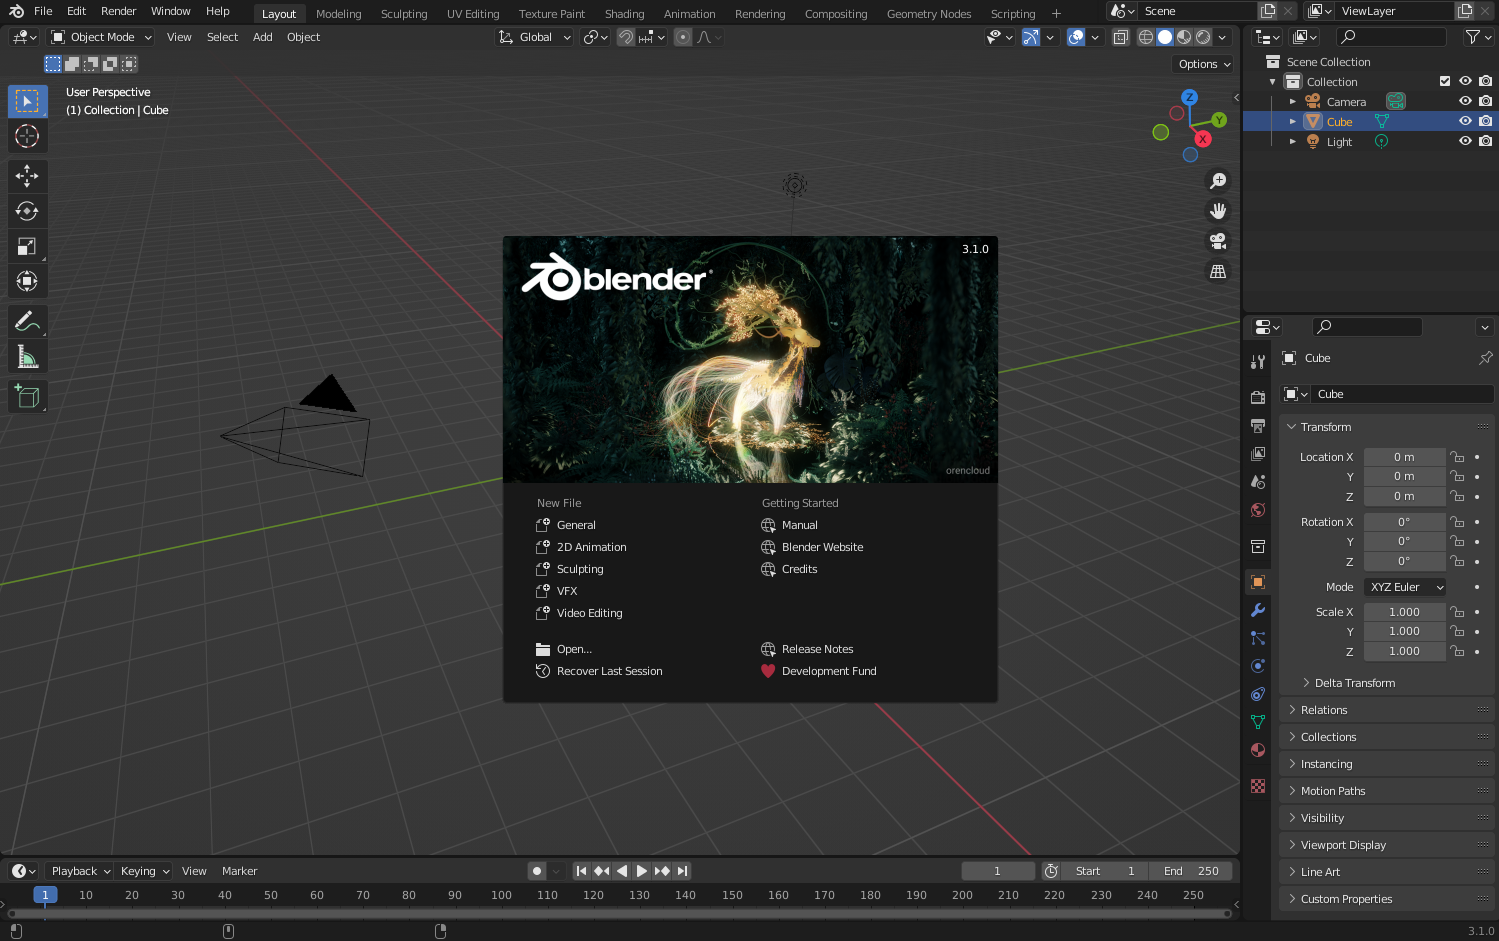
\includegraphics[height=6cm]{figure/Blender_3.1.0_screenshot.png}
    \caption{Interfaccia di Blender 3.1.0}
\end{figure}

Dal lancio del software come open source l'interfaccia utente è cambiata e il motore di render si è evoluto ma le caratteristiche principali sono rimaste invariate.
%
Una delle caratteristiche principali di Blender è che è possibile chiamare quasi tutte le funzioni tramite scorciatoie da tastiera. 
%
Per questo motivo quasi tutti i tasti della tastiera sono associati ad una o più funzioni. 
%
Le funzioni più utilizzate sono associate a tasti che richiamano il nome della funzione che utilizzano, ad esempio il tasto \textit{"G"} chiama la funzione \textit{Grab} che permette di spostare l'elemento selezionato, il tasto \textit{"R"} la funzione \textit{Rotate}, il tasto \textit{"E"} la funzione \textit{Extrude} e così via.

Un'altra caratteristica di Blender è che lo spazio di lavoro è totalmente ad oggetti: l'interfaccia è divisa in finestre che è possibile dividere a loro volta in altre fineste e sottofinestre ognuna delle quali può diventare qualsiasi tipo di vista o immagine che il programma supporta.
%
L'utente può personalizzare la combinazione di finestre e viste per ognuna delle operazioni che preferisce e può posizionare questi layout in schede similmente a come avviene in un browser web.
%
Il programma offre già layout di default per lavorare a compiti diversi. 


    % focus sul progresso tecnologico che resterà nonostante questa sia una bolla finanziaria che scoppierà

    % Metaverso e blockchain hanno ricevuto tantissimi investimenti anche milionari, e sicuramente questo (anche se il mercato delle crypto fallirà) lascerà dei risultati in termini di avanzamento tecnologico

% Pets.com 

% Tedtalk di Talkman premio nobel economia monete e bitcoin

% The line goes up

% Moonekat canale youtube

% Descrizione pura e asettica senza entrare nel dettaglio economico e senza dire che potrà essere una rivoluzione

% Almeno 80 pagine

% .sol per vedere che cos'è uno smart contract

% cosa esce da un'NFT e cosa si vede

